\subsection{Κατανόηση Αλγορίθμου}
Ο αλγόριθμος αυτός βασίζεται στην ακολουθία \selectlanguage{english}Fibonacci\selectlanguage{greek}
μέσω της οποίας ορίζονται διαστήματα αναζήτησης πολύ πιο αποτελεσματικά από τις άλλες μεθόδους. Αυτό 
συμβαίνει επειδή μειώνουμε το διάστημα αναζήτησης κατά $\frac{F_{n-k}}{F_{n-k-1}}$, περισσότερο από όσο
μειωνόταν με τους προηγούμενους αλγορίθμους. Ακόμη, όπως και στον αλγόριθμο της χρυσής τομής εξοικονομούμε
πόρους υπολογίζοντας λιγότερες φορές τις τιμές της εκάστοτε συνάρτησής μας.

\subsection{Υπολογισμοί αντικειμενικής συνάρτησης συναρτήσει του $l$}
\begin{figure}[H] % h for 'here', you can also use t (top), b (bottom), or p (page)
    \centering
    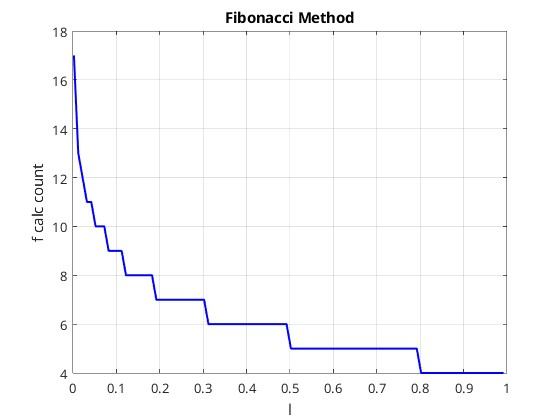
\includegraphics[width=0.5\textwidth]{media/fibonaccif1} % Image file without extension
    \caption{Συνάρτηση $f_1$}
\end{figure}

\begin{figure}[H] % h for 'here', you can also use t (top), b (bottom), or p (page)
    \centering
    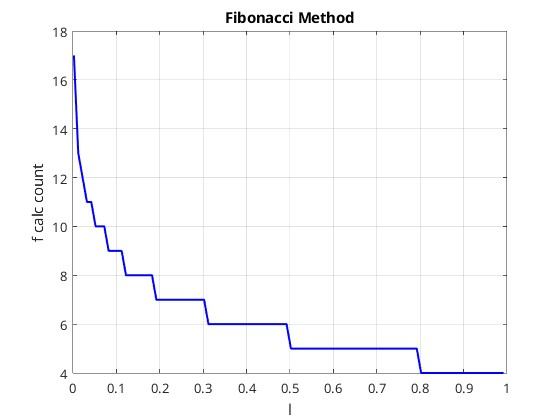
\includegraphics[width=0.5\textwidth]{media/fibonaccif2} % Image file without extension
    \caption{Συνάρτηση $f_2$}
\end{figure}

\begin{figure}[H] % h for 'here', you can also use t (top), b (bottom), or p (page)
    \centering
    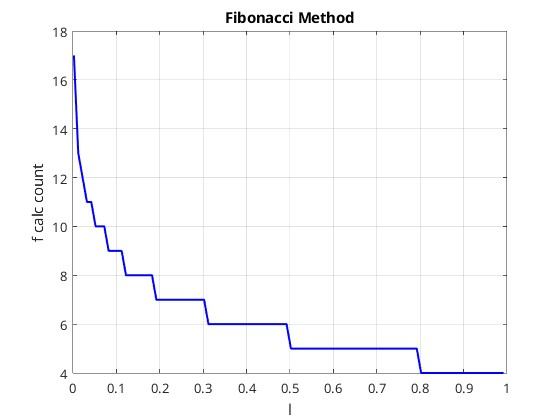
\includegraphics[width=0.5\textwidth]{media/fibonaccif3} % Image file without extension
    \caption{Συνάρτηση $f_3$}
\end{figure}
\subsection{Άκρα του διαστήματος αναζήτησης συναρτήσει του δείκτη επαναλήψεων}
Συνάρτηση $f_1$:
\begin{figure}[H] % h for 'here', you can also use t (top), b (bottom), or p (page)
    \centering
    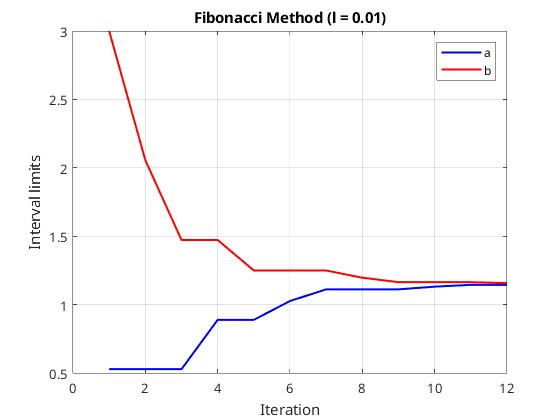
\includegraphics[width=0.5\textwidth]{media/fibonaccif1_001} % Image file without extension
    \caption{Συνάρτηση $f_1$}
\end{figure}
\begin{figure}[H] % h for 'here', you can also use t (top), b (bottom), or p (page)
    \centering
    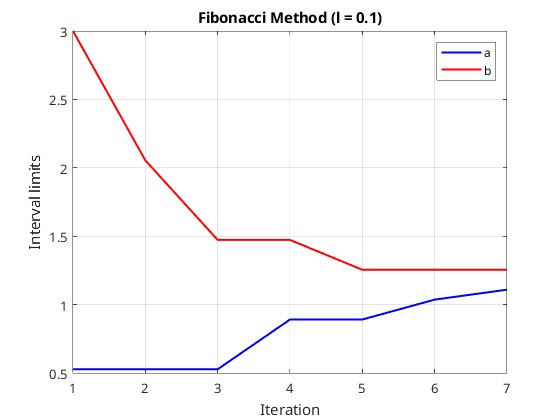
\includegraphics[width=0.5\textwidth]{media/fibonaccif1_01} % Image file without extension
    \caption{Συνάρτηση $f_1$}
\end{figure}
\begin{figure}[H] % h for 'here', you can also use t (top), b (bottom), or p (page)
    \centering
    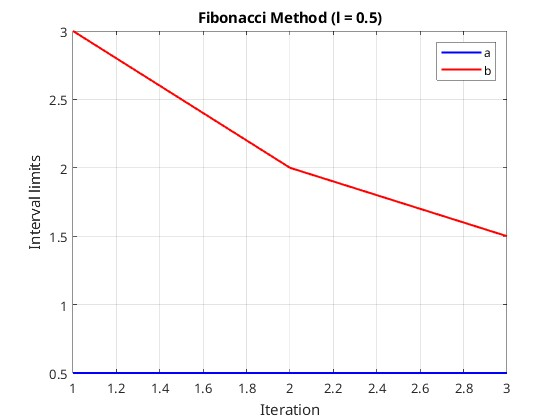
\includegraphics[width=0.5\textwidth]{media/fibonaccif1_05} % Image file without extension
    \caption{Συνάρτηση $f_1$}
\end{figure}

Συνάρτηση $f_2$:
\begin{figure}[H] % h for 'here', you can also use t (top), b (bottom), or p (page)
    \centering
    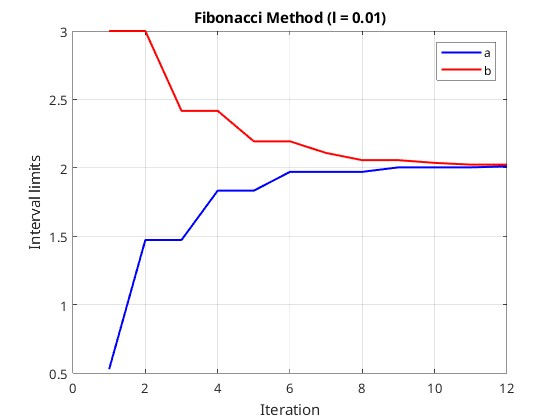
\includegraphics[width=0.5\textwidth]{media/fibonaccif2_001} % Image file without extension
    \caption{Συνάρτηση $f_2$}
\end{figure}
\begin{figure}[H] % h for 'here', you can also use t (top), b (bottom), or p (page)
    \centering
    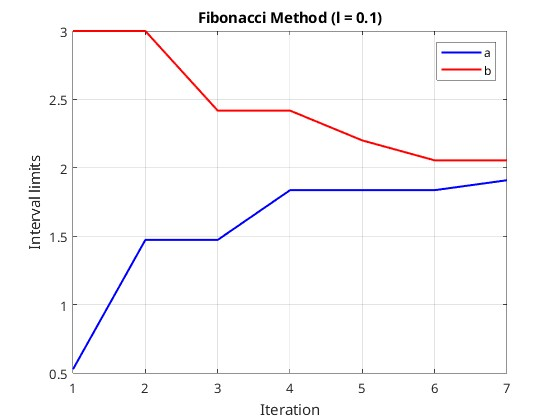
\includegraphics[width=0.5\textwidth]{media/fibonaccif2_01} % Image file without extension
    \caption{Συνάρτηση $f_2$}
\end{figure}
\begin{figure}[H] % h for 'here', you can also use t (top), b (bottom), or p (page)
    \centering
    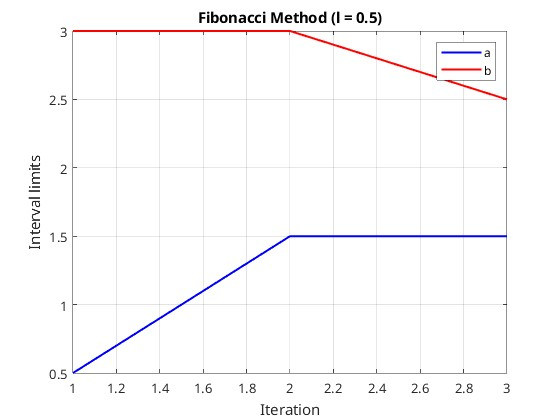
\includegraphics[width=0.5\textwidth]{media/fibonaccif2_05} % Image file without extension
    \caption{Συνάρτηση $f_2$}
\end{figure}

Συνάρτηση $f_3$:
\begin{figure}[H] % h for 'here', you can also use t (top), b (bottom), or p (page)
    \centering
    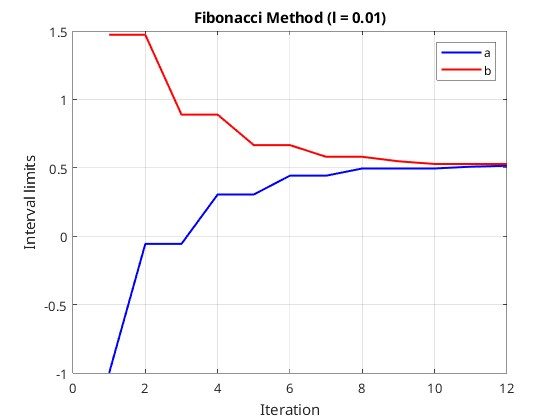
\includegraphics[width=0.5\textwidth]{media/fibonaccif3_001} % Image file without extension
    \caption{Συνάρτηση $f_3$}
\end{figure}
\begin{figure}[H] % h for 'here', you can also use t (top), b (bottom), or p (page)
    \centering
    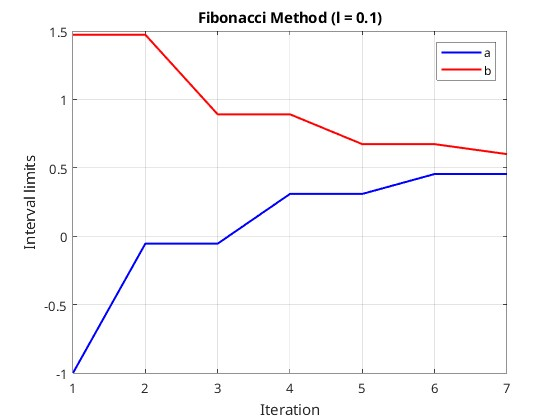
\includegraphics[width=0.5\textwidth]{media/fibonaccif3_01} % Image file without extension
    \caption{Συνάρτηση $f_3$}
\end{figure}
\begin{figure}[H] % h for 'here', you can also use t (top), b (bottom), or p (page)
    \centering
    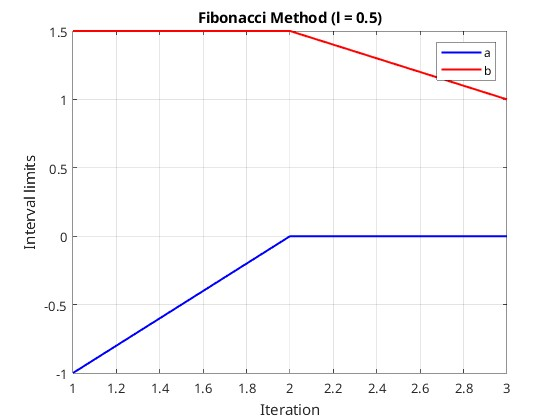
\includegraphics[width=0.5\textwidth]{media/fibonaccif3_05} % Image file without extension
    \caption{Συνάρτηση $f_3$}
\end{figure}